\documentclass[11pt,a4paper]{article}


\usepackage{amssymb,amsmath,amsfonts}    %ams
\usepackage{wasysym} %des symboles
%\usepackage{a4wide}
\usepackage[tmargin=1in,bmargin=1in,lmargin=.75in,rmargin=.75in]{geometry}
\usepackage{graphicx}
%\usepackage{pstricks}
%\usepackage{multido}
\usepackage{verbatim}
\usepackage{enumerate}
\usepackage{tikz}
\usetikzlibrary{calc,positioning,backgrounds}

\usepackage[utf8]{inputenc} 
%\usepackage[T1]{fontenc}
\usepackage{listings}

\newcommand{\R}{{\mathbb R}}   % reals
\newcommand{\Q}{{\mathbb Q}}   % rationals
\newcommand{\N}{{\mathbb N}}   %natural numbers
\newcommand{\Z}{{\mathbb Z}}    %integers
\renewcommand{\P}{{\mathbb P}}   %primes
\newcommand{\F}{{\mathbb F}}

\newcommand\cc{{\cal C}}
\newcommand{\cw}{{\cal W}}



\newtheorem{theorem}{Theorem}
\newtheorem{cor}{Corollary}
\newtheorem{example}{Example}
\newtheorem{lemma}{Lemma}
\newtheorem{newcommandi}{Definition}


\newcommand{\proof}{\noindent {\bf Proof.\ \ }}

\newcommand{\qed}{\hfill $\square$}


\newcommand{\card}[1]{\vert #1 \vert}

%\newcommand{\qed}{\hspace*{\fill} $\Box$ \bigskip }


%\renewcommand{\thefootnote}{\Alph{footnote}}
\usepackage{fancybox}
\usepackage[french]{babel}
%\usepackage{fullpage}
\usepackage{multicol}
\setlength{\columnseprule}{0.2pt}
\setlength{\columnsep}{16pt}
\usepackage{fancyhdr} % personalisation tete/pied de page
%\pagestyle{fancy}







\usepackage{hyperref}

%\addtolength{\headheight}{50pt}

\setlength{\parindent}{0pt}

\title{Fiche 3.0 : scripts et modules}
\author{BUT Informatique\\
IUT de Vélizy\\
}
\date{}


%\catcode`\_=12 %for escaping underscore

\newcommand{\ww}[1]{\textcolor{white}{#1}}

\newcommand{\code}[1]{%
    \begin{center}
        \tt #1
        \vskip .2cm
        {\tt
            \lstinputlisting[frame=single]{#1}
        }
    \end{center}
}


\usepackage{marginnote}

\usepackage{fancyvrb} % Verbatim avancé

\lstdefinestyle{customc}{
    belowcaptionskip=1\baselineskip,
    breaklines=true,
    frame=single,
    xleftmargin=2cm,
    language=C,
    showstringspaces=false,
    showspaces=false,
    basicstyle=\ttfamily
}


\newcommand{\reflexion}{\hspace{-1.2cm} 
\includegraphics[width=1cm]{reflexion.jpg} \vskip -.8cm}
%\newcommand{\checkbox}{
\includegraphics[width=.5cm]{checkbox.jpg} }
\newcommand{\checkbox}{$\square$ \smallskip}


%%environement pour les icones avec decalage
\newenvironment{icone}[1]{%
    \hskip -.8cm
\begin{tabular}{c|c}
    \hspace{.03\textwidth} \includegraphics[width=.07\textwidth]{#1} & 
\begin{minipage}{.85\textwidth}
}{%
\end{minipage}
\end{tabular}
}





\newcounter{exo} \setcounter{exo}{0}
\newenvironment{action}{%
    \begin{enumerate}[\numerotation] \addtocounter{exo}{-1}%
        }{%
    \end{enumerate}
}

%environement pour liste avec checkbox avec compteur
\newcommand{\numexoa}{\theexo \addtocounter{exo}{1}}
\newcommand{\numerotation}{\checkbox \smallskip \numexoa.}

%%environement de validation
\newenvironment{validation}{%
\smallskip
\begin{tabular}{c|c}
    \hspace{.03\textwidth} 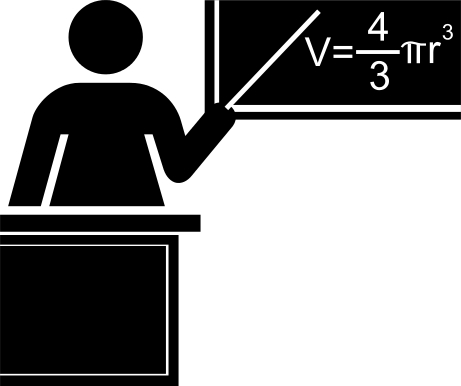
\includegraphics[width=.07\textwidth]{teacher.jpg} & 
\begin{minipage}{.85\textwidth}
}{%
\end{minipage}\\
\hline
\end{tabular}
}


%pour les fichiers c et dossiers
\newcounter{exoo} \setcounter{exoo}{0}
\newcommand{\numexo}{\theexoo}
\newcommand{\repexo}{{\tt exo\_\numexo}}
\newcommand{\exoplus}{\addtocounter{exoo}{1}}




\begin{document}
\maketitle





\thispagestyle{empty}


\section{Notion de script}

\begin{icone}{lecture.jpg}
Jusqu'à présent, vous avez écrit du python dans l'environnement interactif {\it jupyter}. Mais en général les programmes python sont indépendants de ce genre d'environnement et peuvent être exécutés "directement".

Un {\it script} python est simplement un fichier texte, dont l'extension est en général {\tt .py} et qui contient du code. Un programme python est en général un ensemble de scripts.

	En python, un script s'appelle un {\it module}, il y a quelques nuances mais ça ira pour l'instant. Plus de détails dans \url{https://docs.python.org/fr/3/tutorial/modules.html}

Pour écrire un tel script, on peut utiliser un simple {\it éditeur de texte} (gedit, vim, emacs, geany, sublimetext,...) ou un {\it environnement de développement intégré} (IDE) (eclipse, pycharm, jetbrains,vscode,...), qui est un éditeur de texte avec de nombreuses fonctions supplémentaires pour écrire du code.

Dans cette séquence, afin de ne pas tout mélanger, nous utiliserons l'éditeur {\bf geany} qui est très simple. Par la suite, vous ferez comme vous voudrez.
\end{icone}


\section{Prise en main}

\begin{action}
\item Ouvrez l'éditeur de texte {\it geany}. Tapez quelques lignes de code python dans l'éditeur, par exemple effectuez une boucle pour écrire 10 fois "bonjour".
\item Enregistrez dans votre dossier de la sequence3 ce programme sous le nom {\tt first\_script.py}
\item Maintenant, ouvrez un terminal et naviguez en ligne de commande jusqu'à vous trouver dans le répertoire où se trouve le script.
\item Tapez dans la ligne de commande

	\begin{center}
		\tt python3  first\_script.py
		\end{center}
N'oubliez pas que la touche TAB permet de compléter automatiquement. En
principe, vous devriez voir dans le terminal la sortie de votre programme.
Sinon, c'est peut-être que vous avez un message d'erreur. Corrigez le script et recommencez.
\item Retenez la procédure ci-dessus, il faudra toujours la faire pour exécuter
  les programmes python en ligne de commande.
\end{action}

\section{Ecriture d'une librairie {\it todolist} pour gérer les trucs à faire}

\begin{icone}{lecture.jpg}
	Quand vous exécutez le script, python va tout lire et exécuter, dans l'ordre du script, de haut en bas. Quand python tombe sur la définition d'une fonction,({\tt def ...})  il n'exécute pas le code de la fonction, il prend juste note de son existence. Pour vraiment exécuter la fonction, il faut l'appeler !
\end{icone} \\


Vous allez maintenant réaliser un petit module avec quelques fonctions ayant
pour but de gérer une liste de tâches à réaliser ou {\tt todolist}. Plus
précisément, on veut avoir en mémoire un ensemble de tâches à réaliser, avec
trois priorités possibles, comme :

\begin{verbatim}
Tâches priorité haute :
	0. réviser cours dev
	1. appeler Mamie
Tâches priorité moyenne :
	2. vaisselle
Tâches priorité basse :
	3. finir de regarder F&F 42
	4. réviser encore cours dev
\end{verbatim}

Vous pouvez imaginer autre chose et faire des variations plus avancées sur ce
principe (possibilité de prévoir des tâches à des dates fixées, plus de
priorités, etc.)

\begin{action}
\item Créez deux scripts, {\tt todolist.py} et {\tt test\_todo.py}.
  \begin{itemize}
  \item Le premier contiendra l'ensemble des fonctions pour manipuler la
    todolist, et uniquement des fonctions destinées à être utilisées par un
    programme. Il s'agit d'une librairie, un
    ensemble de fonctions destinées à gérer les todolist. Si on exécute ce
    script directement en ligne de commande, rien ne se passera car aucune des
    fonctions
    n'est appelée, il n'y a pas de code principal.
  \item le second script contient des tests destinés à vérifier si nos
    fonctions de l'autre script sont bien écrites. Après les
    fonctions de test, le code principal de ce script lance les tests.
  \end{itemize} 
\item A vous de décider comment vous allez gérer la sauvegarde des tâches et
  leur priorité : plusieurs listes, dictionnaire de listes, liste de listes ... A
  vous de faire au mieux, au plus simple et surtout au plus efficace !
  Toutes les fonctions que vous allez écrire devront
  avoir ces objets en paramètre.


\item  On va créeer, dans le script {\tt todolist.py}, une fonction destinée à
  afficher la liste des tâches comme ci-dessus. Ecrivez le {\it prototype} de
  cette fonction : le mot clé {\tt def}, le nom de la fonction, et pour
  l'instant
  ne mettez pas de code (juste {\tt pass}).

\item Ecrivez maintenant la spécification de la fonction en docstring : que
  sont les paramètres, que fait la fonction, qu'est-ce qu'elle renvoie ?
  Respectez     le format utilisé dans la séquence précédente.

\item Dans le script {\tt test\_todo.py}, qui doit se trouver dans le même
  répertoire, écrivez {\tt import todolist} avant votre code. Ceci permettra
  d'utiliser les fonctions de l'autre script dans celui-ci. Ecrivez
  maintenant une fonction de test de votre affichage : il faut
  créer (\og à la main\fg pour l'instant) une liste de tâches au format
  que vous avez choisi, appeler la fonction d'affichage en lui donnant
  cette liste en paramètre. Faites aussi un test pour un cas où il n'y a pas
  de tâches à afficher. En principe, cette fonction de test ne prends pas de
  paramètres.

  note : on ne peut pas faire un {\tt assert} pour vérifier l'affichage.
  Il faudra regarder avec nos yeux si ça correspond bien à ce qu'on veut.

\item Il est temps d'écrire maintenant la fonction d'affichage ! Supprimez
  {\tt pass} et écrivez le code.

\item Dans le script de tests, en dessous des fonction de tests, écrivez
  le \og code principal\fg de ce script (ou {\it main}) : il s'agit juste
  d'un appel à votre fonction de test.

\item Maintenant, en ligne de commande, lancez votre script de tests. La
  dernière ligne est exécutée : elle appelle la fonction de test, qui
  elle même appelle la fonction de d'affichage du script {\tt
    todolist.py}.
  Si tout se passe bien, l'affichage a lieu. Sinon, il doit y avoir un
  bug quelque part !

\item Respectez scrupuleusement les mêmes étapes (spécification, test,
  développement) pour l'écriture d'une
  fonction qui permet d'ajouter une nouvelle tâche dans la todolist. Attention,
  cette fonction ne lit pas de saisie au clavier.

\item Idem pour supprimer une tâche, pour changer la priorité d'une tâche, et toute autre fonction que vous pourrez imaginer qui pourrait servir dans votre librairie.

\item Ecrivez un test complet de votre librairie : cela crée une todolist, ajoute quelques tâches, les affiche, supprime et ajoute d'autres tâches, affiche, etc.
\end{action}




\end{document}
